\documentclass[12pt]{article}

\author{Matthew D. Cocci}
\title{Microeconomics}
\date{\today}

%% Formatting & Spacing %%%%%%%%%%%%%%%%%%%%%%%%%%%%%%%%%%%%

%\usepackage[top=1in, bottom=1in, left=1in, right=1in]{geometry} % most detailed page formatting control
\usepackage{fullpage} % Simpler than using the geometry package; std effect
\usepackage{setspace}
%\onehalfspacing
\usepackage{microtype}

%% Formatting %%%%%%%%%%%%%%%%%%%%%%%%%%%%%%%%%%%%%%%%%%%%%

%\usepackage[margin=1in]{geometry}
    %   Adjust the margins with geometry package
%\usepackage{pdflscape}
    %   Allows landscape pages
%\usepackage{layout}
    %   Allows plotting of picture of formatting



%% Header %%%%%%%%%%%%%%%%%%%%%%%%%%%%%%%%%%%%%%%%%%%%%%%%%

%\usepackage{fancyhdr}
%\pagestyle{fancy}
%\lhead{}
%\rhead{}
%\chead{}
%\setlength{\headheight}{15.2pt}
    %   Make the header bigger to avoid overlap

%\fancyhf{}
    %   Erase header settings

%\renewcommand{\headrulewidth}{0.3pt}
    %   Width of the line

%\setlength{\headsep}{0.2in}
    %   Distance from line to text


%% Mathematics Related %%%%%%%%%%%%%%%%%%%%%%%%%%%%%%%%%%%

\usepackage{amsmath}
\usepackage{amssymb}
\usepackage{amsfonts}
\usepackage{mathrsfs}
\usepackage{amsthm} %allows for labeling of theorems
%\numberwithin{equation}{section} % Number equations by section
\usepackage{bbm} % For bold numbers

\theoremstyle{plain}
\newtheorem{thm}{Theorem}[section]
\newtheorem{lem}[thm]{Lemma}
\newtheorem{prop}[thm]{Proposition}
\newtheorem{cor}[thm]{Corollary}

\theoremstyle{definition}
\newtheorem{defn}[thm]{Definition}
\newtheorem{ex}[thm]{Example}
\newtheorem{ax}[thm]{Axiom}


\theoremstyle{remark}
\newtheorem*{rmk}{Remark}
\newtheorem*{note}{Note}

% Below supports left-right alignment in matrices so the negative
% signs don't look bad
\makeatletter
\renewcommand*\env@matrix[1][c]{\hskip -\arraycolsep
  \let\@ifnextchar\new@ifnextchar
  \array{*\c@MaxMatrixCols #1}}
\makeatother


%% Font Choices %%%%%%%%%%%%%%%%%%%%%%%%%%%%%%%%%%%%%%%%%

\usepackage[T1]{fontenc}
\usepackage{lmodern}
\usepackage[utf8]{inputenc}
%\usepackage{blindtext}
\usepackage{courier}


%% Figures %%%%%%%%%%%%%%%%%%%%%%%%%%%%%%%%%%%%%%%%%%%%%%

\usepackage{tikz}
\usetikzlibrary{decorations.pathreplacing}
\usepackage{graphicx}
\usepackage{subfigure}
    %   For plotting multiple figures at once
%\graphicspath{ {Directory/} }
    %   Set a directory for where to look for figures


%% Hyperlinks %%%%%%%%%%%%%%%%%%%%%%%%%%%%%%%%%%%%%%%%%%%%
\usepackage{hyperref}
\hypersetup{%
    colorlinks,
        %   This colors the links themselves, not boxes
    citecolor=black,
        %   Everything here and below changes link colors
    filecolor=black,
    linkcolor=black,
    urlcolor=black
}

%% Colors %%%%%%%%%%%%%%%%%%%%%%%%%%%%%%%%%%%%%%%%%%%%%%%

\usepackage{color}
\definecolor{codegreen}{RGB}{28,172,0}
\definecolor{codelilas}{RGB}{170,55,241}

% David4 color scheme
\definecolor{d4blue}{RGB}{100,191,255}
\definecolor{d4gray}{RGB}{175,175,175}
\definecolor{d4black}{RGB}{85,85,85}
\definecolor{d4orange}{RGB}{255,150,100}

%% Including Code %%%%%%%%%%%%%%%%%%%%%%%%%%%%%%%%%%%%%%%

\usepackage{verbatim}
    %   For including verbatim code from files, no colors
\usepackage{listings}
    %   For including code snippets written directly in this doc

\lstdefinestyle{bash}{%
  language=bash,%
  basicstyle=\footnotesize\ttfamily,%
  showstringspaces=false,%
  commentstyle=\color{gray},%
  keywordstyle=\color{blue},%
  xleftmargin=0.25in,%
  xrightmargin=0.25in
}

\lstdefinestyle{matlab}{%
  language=Matlab,%
  basicstyle=\footnotesize\ttfamily,%
  breaklines=true,%
  morekeywords={matlab2tikz},%
  keywordstyle=\color{blue},%
  morekeywords=[2]{1}, keywordstyle=[2]{\color{black}},%
  identifierstyle=\color{black},%
  stringstyle=\color{codelilas},%
  commentstyle=\color{codegreen},%
  showstringspaces=false,%
    %   Without this there will be a symbol in
    %   the places where there is a space
  numbers=left,%
  numberstyle={\tiny \color{black}},%
    %   Size of the numbers
  numbersep=9pt,%
    %   Defines how far the numbers are from the text
  emph=[1]{for,end,break,switch,case},emphstyle=[1]\color{red},%
    %   Some words to emphasise
}

\newcommand{\matlabcode}[1]{%
    \lstset{style=matlab}%
    \lstinputlisting{#1}
}
    %   For including Matlab code from .m file with colors,
    %   line numbering, etc.

%% Bibliographies %%%%%%%%%%%%%%%%%%%%%%%%%%%%%%%%%%%%

%\usepackage{natbib}
    %---For bibliographies
%\setlength{\bibsep}{3pt} % Set how far apart bibentries are

%% Misc %%%%%%%%%%%%%%%%%%%%%%%%%%%%%%%%%%%%%%%%%%%%%%

\usepackage{enumitem}
    %   Has to do with enumeration
\usepackage{appendix}
%\usepackage{natbib}
    %   For bibliographies
\usepackage{pdfpages}
    %   For including whole pdf pages as a page in doc


%% User Defined %%%%%%%%%%%%%%%%%%%%%%%%%%%%%%%%%%%%%%%%%%

%\newcommand{\nameofcmd}{Text to display}
\newcommand*{\Chi}{\mbox{\large$\chi$}} %big chi
    %   Bigger Chi

% In math mode, Use this instead of \munderbar, since that changes the
% font from math to regular
\makeatletter
\def\munderbar#1{\underline{\sbox\tw@{$#1$}\dp\tw@\z@\box\tw@}}
\makeatother

% Misc Math
\newcommand{\ra}{\rightarrow}
\newcommand{\diag}{\text{diag}}
\newcommand{\ch}{\text{ch}}
\newcommand{\dom}{\text{dom}}
\newcommand{\one}[1]{\mathbf{1}_{#1}}


% Script
\newcommand{\sF}{\mathscr{F}}
\newcommand{\sB}{\mathscr{B}}
\newcommand{\sL}{\mathscr{L}}
\newcommand{\sM}{\mathscr{M}}
\newcommand{\sT}{\mathscr{T}}
\newcommand{\sA}{\mathscr{A}}
\newcommand{\sP}{\mathscr{P}}

% Boldsymbol
\newcommand{\bsb}{\boldsymbol{b}}
\newcommand{\bshatb}{\boldsymbol{\hat{b}}}
\newcommand{\bsd}{\boldsymbol{d}}
\newcommand{\bsg}{\boldsymbol{g}}
\newcommand{\bsG}{\boldsymbol{G}}
\newcommand{\bsJ}{\boldsymbol{J}}
\newcommand{\bsh}{\boldsymbol{h}}
\newcommand{\bsS}{\boldsymbol{S}}
\newcommand{\bsu}{\boldsymbol{u}}
\newcommand{\bsx}{\boldsymbol{x}}
\newcommand{\bsX}{\boldsymbol{X}}
\newcommand{\bsy}{\boldsymbol{y}}
\newcommand{\bsY}{\boldsymbol{Y}}
\newcommand{\bstheta}{\boldsymbol{\theta}}
\newcommand{\bsmu}{\boldsymbol{\mu}}
\newcommand{\bsSigma}{\boldsymbol{\Sigma}}
\newcommand{\bshatmu}{\boldsymbol{\hat{\mu}}}
\newcommand{\bshatSigma}{\boldsymbol{\hat{\Sigma}}}

% Transposes of all the boldsymbol shit
\newcommand{\bsbp}{\boldsymbol{b'}}
\newcommand{\bshatbp}{\boldsymbol{\hat{b'}}}
\newcommand{\bsdp}{\boldsymbol{d'}}
\newcommand{\bsgp}{\boldsymbol{g'}}
\newcommand{\bsGp}{\boldsymbol{G'}}
\newcommand{\bshp}{\boldsymbol{h'}}
\newcommand{\bsSp}{\boldsymbol{S'}}
\newcommand{\bsup}{\boldsymbol{u'}}
\newcommand{\bsxp}{\boldsymbol{x'}}
\newcommand{\bsyp}{\boldsymbol{y'}}
\newcommand{\bsthetap}{\boldsymbol{\theta'}}
\newcommand{\bsmup}{\boldsymbol{\mu'}}
\newcommand{\bsSigmap}{\boldsymbol{\Sigma'}}
\newcommand{\bshatmup}{\boldsymbol{\hat{\mu'}}}
\newcommand{\bshatSigmap}{\boldsymbol{\hat{\Sigma'}}}

% Mathcal
\newcommand{\calA}{\mathcal{A}}
\newcommand{\calB}{\mathcal{B}}
\newcommand{\calC}{\mathcal{C}}
\newcommand{\calD}{\mathcal{D}}
\newcommand{\calE}{\mathcal{E}}
\newcommand{\calF}{\mathcal{F}}
\newcommand{\calG}{\mathcal{G}}
\newcommand{\calH}{\mathcal{H}}
\newcommand{\calI}{\mathcal{I}}
\newcommand{\calL}{\mathcal{L}}
\newcommand{\calM}{\mathcal{M}}
\newcommand{\calN}{\mathcal{N}}
\newcommand{\calP}{\mathcal{P}}

% Dot over
\newcommand{\dx}{\dot{x}}
\newcommand{\ddx}{\ddot{x}}
\newcommand{\dy}{\dot{y}}
\newcommand{\ddy}{\ddot{y}}

% First derivatives
\newcommand{\dydx}{\frac{dy}{dx}}
\newcommand{\dfdx}{\frac{df}{dx}}
\newcommand{\dfdy}{\frac{df}{dy}}
\newcommand{\dfdz}{\frac{df}{dz}}

% Second derivatives
\newcommand{\ddyddx}{\frac{d^2y}{dx^2}}
\newcommand{\ddydxdy}{\frac{d^2y}{dx dy}}
\newcommand{\ddydydx}{\frac{d^2y}{dy dx}}
\newcommand{\ddfddx}{\frac{d^2f}{dx^2}}
\newcommand{\ddfddy}{\frac{d^2f}{dy^2}}
\newcommand{\ddfddz}{\frac{d^2f}{dz^2}}
\newcommand{\ddfdxdy}{\frac{d^2f}{dx dy}}
\newcommand{\ddfdydx}{\frac{d^2f}{dy dx}}

% First Partial Derivatives
\newcommand{\pypx}{\frac{\partial y}{\partial x}}
\newcommand{\pfpx}{\frac{\partial f}{\partial x}}
\newcommand{\pfpy}{\frac{\partial f}{\partial y}}
\newcommand{\pfpz}{\frac{\partial f}{\partial z}}


% Blackboard
\newcommand{\R}{\mathbb{R}}
\newcommand{\Rn}{\mathbb{R}^n}
\newcommand{\Rk}{\mathbb{R}^n}
\newcommand{\Rnn}{\mathbb{R}^{n\times n}}
\newcommand{\C}{\mathbb{C}}
\newcommand{\Cn}{\mathbb{C}^n}
\newcommand{\Cnn}{\mathbb{C}^{n\times n}}
\newcommand{\N}{\mathbb{N}}
\newcommand{\Q}{\mathbb{Q}}
\newcommand{\Z}{\mathbb{Z}}
\newcommand{\E}{\mathbb{E}}

\DeclareMathOperator*{\argmin}{arg\;min}
\DeclareMathOperator*{\argmax}{arg\;max}
\newenvironment{rcases}
  {\left.\begin{aligned}}
  {\end{aligned}\right\rbrace}

% Various probability and statistics commands
\newcommand{\Prb}{\mathrm{P}}
\newcommand{\Cov}{\operatorname{Cov}}
\newcommand{\Corr}{\operatorname{Corr}}
\newcommand{\Var}{\operatorname{Var}}
\newcommand{\asto}{\xrightarrow{a.s.}}
\newcommand{\pto}{\xrightarrow{p}}
\newcommand{\msto}{\xrightarrow{m.s.}}
\newcommand{\dto}{\xrightarrow{d}}
\newcommand{\Lpto}{\xrightarrow{L_p}}
\newcommand{\plim}{\text{plim}_{n\rightarrow\infty}}
\newcommand{\W}{\Omega}
\newcommand{\w}{\omega}


% Redefine real and imaginary from fraktur to plain text
\renewcommand{\Re}{\operatorname{Re}}
\renewcommand{\Im}{\operatorname{Im}}


% Bounds/Limits
\newcommand{\atob}{_a^b}
\newcommand{\ztoinf}{_0^\infty}
\newcommand{\kinf}{_{k=1}^\infty}
\newcommand{\ninf}{_{n=1}^\infty}
\newcommand{\minf}{_{m=1}^\infty}
\newcommand{\kinfz}{_{k=0}^\infty}
\newcommand{\ninfz}{_{n=0}^\infty}
\newcommand{\minfz}{_{m=0}^\infty}


% Shorter sums: ``Sum from X to Y''
% - sumXY  is equivalent to \sum^Y_{X=1}
% - sumXYz is equivalent to \sum^Y_{X=0}
\newcommand{\sumnN}{\sum_{n=1}^N}
\newcommand{\sumin}{\sum_{i=1}^n}
\newcommand{\sumkn}{\sum_{k=1}^n}
\newcommand{\sumtT}{\sum_{t=1}^T}
\newcommand{\sumninf}{\sum_{n=1}^\infty}
\newcommand{\sumtinf}{\sum_{t=1}^\infty}
\newcommand{\sumnNz}{\sum_{n=0}^N}
\newcommand{\suminz}{\sum_{i=0}^n}
\newcommand{\sumknz}{\sum_{k=0}^n}
\newcommand{\sumtTz}{\sum_{t=0}^T}
\newcommand{\sumninfz}{\sum_{n=0}^\infty}
\newcommand{\sumtinfz}{\sum_{t=0}^\infty}

% Limits
\newcommand{\limN}{\lim_{N\rightarrow\infty}}
\newcommand{\limn}{\lim_{n\rightarrow\infty}}
\newcommand{\limk}{\lim_{k\rightarrow\infty}}
\newcommand{\limt}{\lim_{t\rightarrow\infty}}
\newcommand{\limT}{\lim_{T\rightarrow\infty}}
\newcommand{\limhz}{\lim_{h\rightarrow 0}}



%%%%%%%%%%%%%%%%%%%%%%%%%%%%%%%%%%%%%%%%%%%%%%%%%%%%%%%%%%%%%%%%%%%%%%%%
%% BODY %%%%%%%%%%%%%%%%%%%%%%%%%%%%%%%%%%%%%%%%%%%%%%%%%%%%%%%%%%%%%%%%
%%%%%%%%%%%%%%%%%%%%%%%%%%%%%%%%%%%%%%%%%%%%%%%%%%%%%%%%%%%%%%%%%%%%%%%%


\begin{document}
\maketitle
\tableofcontents


\clearpage
\section{Preferences and Utility}

\subsection{Binary Relations}

\begin{defn}(Binary Relation)
A \emph{binary relation} $R$ on a set $X$ is a subset of $X\times X$. We
introduce the notation
\begin{align*}
  xRy
  \quad\iff\quad
  (x,y) \in X \times X
\end{align*}
\end{defn}

\begin{ex}
Below is a plot showing two binary relations on $\R$. Relation $R_1$ is
the dashed line, the subset of $\R^2$ such that $x=y$. Relation $R_2$ is
includes the elements of $R_1$ and all elements above the line. It
captures the subset of $\R^2$ such that $y\geq x$.

In fact, in the context of relations, statements like $x=y$, $x\leq y$,
$xRy$, $x\succeq y$ should not first be thought of as ``true or false''
statements. Rather, they should be thought of as conditions tracing out
or identifying subsets of the underlying space $X$.
\begin{figure}[htpb!]
\centering
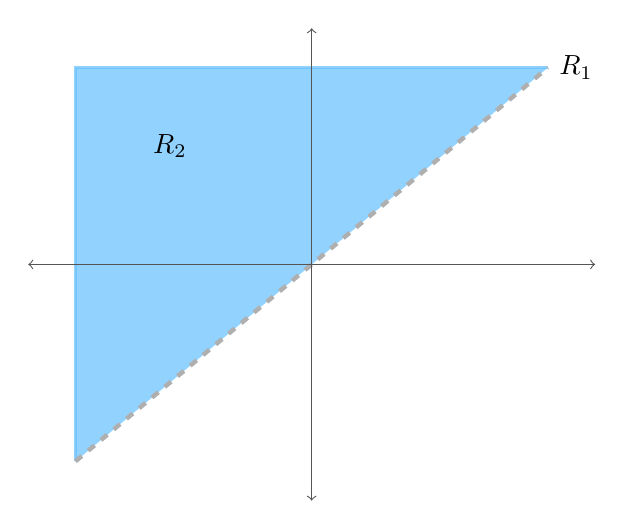
\begin{tikzpicture}[xscale=1.2]
  \draw[d4blue, thick, fill=d4blue, opacity=0.7] %
    (-2.5,-2.5) -- (-2.5,2.5) -- (2.5,2.5);
  \draw node at (-1.5,1.5) {$R_2$};
  \draw[d4gray, ultra thick, dashed] %
    (-2.5,-2.5) -- (2.5,2.5) node[black, right] {$R_1$};
  \draw[d4black, <->] (-3,0) -- (3,0);
  \draw[d4black, <->] (0,-3) -- (0,3);
\end{tikzpicture}
\end{figure}
\end{ex}

\begin{defn}(Properties of Relations)
Given binary relation $R$ over $X$ and given $x,y,z\in X$, we might use
the following terms to describe $R$:
\begin{enumerate}
  \item \emph{Reflexive}: $xRx$ for all $x\in X$
  \item \emph{Complete}: $xRy$ or $yRx$ (or both) for all $x\in X$.
  \item \emph{Transitive}: $xRy$ and $yRz$ implies $xRz$.
  \item \emph{Irreflexive}: $xRx$ never holds. Example: $x>y$
  \item \emph{Symmetric}: $xRy$ implies $yRx$
  \item \emph{Asymmetric}: $xRy$ implies not $yRx$. Example: $x>y$
  \item \emph{Antisymmetric}: $xRy$ and $yRx$ implies $x=y$
\end{enumerate}
\end{defn}

\begin{defn}(Derived Binary Relations)
Given binary relation $\succeq$, define
\begin{align*}
  x \succ y
  \quad&\iff\quad
  \text{both} \;
  \begin{cases}
    x &\succeq y \\
    y &\not\succeq x \\
  \end{cases} \\
  x \sim y
  \quad&\iff\quad
  \text{both} \;
  \begin{cases}
    x &\succeq y \\
    y &\succeq x \\
  \end{cases} \\
\end{align*}
\end{defn}

\begin{defn}(Rational Binary Relation or Preference Relation)
We call a binary relation $R$ on $X$ \emph{rational} or simply a
\emph{preference relation} if $R$ is complete and transitive.
\end{defn}


\subsection{Choice Functions}

In this section, let $\calP(X)$ represent all subsets of $X$
\emph{except} for the emptyset. So if $\sP(X)$ is the power set for $X$,
we define $\calP(X):=\sP(X)\setminus \emptyset$.

\begin{defn}(Choice Function and Choice Structure)
Given a set $X$ and $\calB$, a collection of nonempty subsets of $X$, a
\emph{choice function} or \emph{choice correspondence} is a function
\begin{align*}
  c: \calP(X) \ra \calP(X)
  \quad\text{such that}\quad
  c(B) \subseteq B \qquad \forall B\in\calP(X)
\end{align*}
It takes a nonempty subset of $X$ and returns a nonempty subset of $X$.
If $c(B)$ is a singleton for all $\calP(X)$, we say that $c$ is
\emph{single-valued}.
\\
\\
A \emph{choice structure} is the pair $(\calB,c)$. If no $\calB$ is
specified, it's generally assumed $\calP(X)$.
\end{defn}

\begin{defn}(MWG WARP)
A choice structure $(\calB,c)$ satisfies the
\emph{weak axiom of revealed preference} (WARP) if
\begin{align*}
  \begin{rcases}
    x,y &\in B,B' \\
    x &\in c(B) \\
    y &\in c(B')
  \end{rcases}
  \implies
  x \in c(B')
\end{align*}
In words, if $x$ and $y$ are alternatives in both $B$ and $B'$, choosing
$x$ from set $B$ (when $y$ was avaialble) means that you should also
choose $x$ if you pick $y$ from $B'$.
\end{defn}

\begin{defn}(Faruk Gul WARP)
$c(A)\cap B\neq \emptyset$ implies $c(B)\cap A\subseteq c(A)$
\end{defn}

\begin{defn}(Faruk Gul $\alpha$ and $\beta$ properties)
A choice structure $(\calB,c)$ may or may not satisfy the following
properties
\begin{enumerate}
  \item Property $\alpha$: $c(A\cup B) \cap A \subseteq c(A)$

  \item Property $\beta$: $c(A\cup B) \cap B\neq\emptyset$ implies
    $c(B)\subseteq c(A\cup B)$.
\end{enumerate}
\end{defn}

\begin{ex}
Let $A$ represent the contestants in a wine competition limited to
California wine only. Let $B$ represent the contestants in a wine
competition that accepts competitors worldwide. There might be
contestants in $A$ that are not in $B$ and vice versa.

Faruk Gul's WARP says that if the winners from the California-only wine
competition $c(A)$ are entered into the world competietion---i.e.
$c(A)\cap B\neq \emptyset$---then any winner of the world competition
$c(B)$ that was also entered in the California competition---i.e.  $c(B)
\cap A$---has to be a California competition winner, i.e. in $c(A)$.

Faruk Gul's $\alpha$ property says that adding the world wide
competition contestants into the mix shouldn't change your preferences
over those contestants in the California-only wine competition.

Faruk Gul's $\beta$ property says that if you combine the two
competitions, choose the best, and the best is in the worldwide
competition, the best in the worldwide competition must have won
in the combined competition.
\end{ex}

\begin{prop}
Choice function $c$ satisfies Properties $\alpha$ and $\beta$ iff $c$
satisfies WARP.
\end{prop}

\begin{prop}
If $c$ is a single-valued choice function, satisfying either $\alpha$ or
$\beta$ implies $c$ satisfies WARP.
\end{prop}


\begin{defn}(Choice Function $c_R$ Generated by $R$)
Suppose that $R$ is a binary relation on $R$ (not neccessarily rational,
so not necessarily a preference relation). Then define function
\begin{align*}
  c_R: \calP(X) \ra \calP(X)\cup\emptyset
\end{align*}
such that
\begin{align*}
  c_R(A) = \{x\in A\;|\; xRy \quad\forall y\in A\}
\end{align*}
Note that $c_R$ is not necessarily a choice function since it could map
to $\emptyset$, which violates the definition of a choice function.
\end{defn}

\begin{prop}
If $c_R$ is a choice function (i.e., if it does not return the
emptyset), then it satisfies Property $\alpha$.
\end{prop}

\begin{defn}(Binary Relation $R_c$ Generated by $c$)
Given a choice function $c$, define binary relation $R_c$ as
\begin{align*}
  xR_c y \quad\iff\quad
  x \in c(\{x,y\})
\end{align*}
\end{defn}

\begin{defn}(MWG Revealed Preference Relation)
Given choice structure $(\calB, c)$, the revealed preference relation
$\succeq^*$ is defined
\begin{align*}
  x \succeq^* y
  \quad\iff\quad
  \exists B\in\calB\;\; \text{s.t. both}\;
  \begin{cases}
    x,y\in B \\
    x\in c(B)
  \end{cases}
\end{align*}
Note that this need not be rational.
\end{defn}



\subsection{Utility Functions}

\begin{defn}(Utility Representation)
We say that a utility function $u: X\ra \R$ represents preference
relation $\succeq$ (a rational binary relation) on set $X$ if
\begin{align*}
  x\succeq y
  \quad\iff\quad
  u(x) \geq u(y)
  \qquad\forall x,y\in X
\end{align*}
\end{defn}

\begin{prop}(Non-Uniqueness of Utility Representation)
Given utility function $u$ representing preference relation $\succeq$,
utility function $v$ also represents $\succeq$ iff
there exists a \emph{strictly} increasing (aka strictly monotonic)
function $f:\R\ra\R$ such that
\begin{align*}
  v = f \circ u
\end{align*}
\end{prop}

\begin{defn}(Cardinal and Ordinal Properties)
Any aspect of utility function $u$ that is preserved under strictly
monotonic transformations is called an \emph{ordinal} property.  Any
aspect that is not preserved (like the level of utility $u(x)$) is
called a \emph{cardinal} property.
\end{defn}


\subsection{Rationality Results}

\begin{lem}
Given preference relation (rational binary relation) $\succeq$, we have
\begin{enumerate}
  \item $\succ$ irreflexive and transitive
  \item $\sim$ reflexive, symmetric, and transitive
  \item $x\succeq y \succeq z$ and one of the relations strict, then
    $x\succ z$.
\end{enumerate}
\end{lem}

\begin{prop}
If $R$ is a rational binary relation over finite $X$, then the choice
function $c_R$ generated by $R$ together with nonempty
$\calB\subseteq\calP(X)$ forms a choice structure.
\end{prop}

\begin{prop}
If $R$ is a binary relation over finite $X$, then $(\calP(X),c_R)$
satisfies WARP iff $R$ rational.
\end{prop}

\begin{prop}
If $(\calP(X),c)$ is a choice structure satisfying WARP, $R_c$ is a
rational binary relation.
\end{prop}

\begin{prop}
Choice structure $(\calP(X),c)$ satisfies WARP iff there exists a
rational preference relation $R$ such that $c=c_R$.
\end{prop}

\begin{prop}
\emph{(Rationality as Necessary Condition of Utility Rep.)}
A binary relation $\succeq$ has a utility representation only if
it is rational (complete and transitive).
\end{prop}

\begin{prop}
\emph{(Rational Preferences over a Finite Set have a Utility Rep.)}
Given rational binary relation $R$ over finite set $X$, there exists a
utility function $u$ representing $R$.
\end{prop}

\begin{prop}
For any finite $X$ and binary relation $R$ on $X$, the following three
conditions are equivalent
\begin{enumerate}
  \item $R$ rational
  \item $c_R$ on $\calP(X)$ satisfies WARP
  \item There exists a utility representation of $R$
\end{enumerate}
\end{prop}





\clearpage
\section{Demand Theory}

\subsection{Preferences over Consumption Bundles}

Let $X=\R^L_+$ be the consumption set where $x_i$ is the quantity of the
$i$th good.

\begin{defn}(Upper and Lower Contour Sets)
Given preference relation $\succeq$ over set $X$ and point $x\in X$,
define the \emph{upper} and \emph{lower contour sets} $C_U(x)$ and
$C_L(x)$ as
\begin{align*}
  C_U(x) &= \left\{ y \in X \;|\; y \succeq x \right\} \\
  C_L(x) &= \left\{ y \in X \;|\; x \succeq y \right\} \\
\end{align*}
\end{defn}

\begin{defn}(Describing Preferences over $X$)
Given preference relation $\succeq$ over elements of $X$, we define the
following concepts:
\begin{enumerate}
  \item \emph{Monotone}:
    $x_i \geq y_i$ for all $i$ implies $x \succeq y$
  \item \emph{Monotone*} or \emph{MWG Monotone:}
    $x_i > y_i$ for all $i$ implies $x \succ y$.
  \item \emph{Strongly Monotone}: $x_i\geq y_i$ for all $i$ and
    $x\neq y$ implies that $x\succ y$.

  \item \emph{Locally Nonsatiated}: For all $x\in X$ and
    $\varepsilon>0$, there exists a $y$ such that $||x-y||\leq
    \varepsilon$ and $y\succ x$. This rules out thick indifference
    curves.

  \item \emph{Convex}: $x \succeq y$ implies that
    $\alpha x + (1-\alpha) y \succeq y$ for all $\alpha\in[0,1]$.
    In other words, the upper contour set is convex.
    This reflects diminishing marginal rates of substitution.

  \item \emph{Strictly Convex}: $x \succeq y$ and $x\neq y$ implies that
    $\alpha x + (1-\alpha) y \succ y$ for all $\alpha\in(0,1)$.
\end{enumerate}
\end{defn}


\begin{defn}(Continuity of Preferences)
Given preference relation $\succeq$ over elements of $X$, we give the
following definitions of continuity of preferences:
\begin{enumerate}
  \item \emph{Faruk}: For all $x\succ y$, there exists an
    $\varepsilon>0$ such that
    \begin{align*}
      \begin{rcases}
      ||x-w||<\varepsilon \\
      ||y-z||<\varepsilon
      \end{rcases}
      \implies
      w \succ z
    \end{align*}
  \item \emph{MWG}: For any sequence $\{(x_n,y_n)\}$
    converging to $(x,y)$ such that $x_n\succeq y_n$ for all $n$, we
    also have $x\succeq y$.
  \item \emph{Contour Sets}: The upper and lower countour sets of
    $\succeq$ are closed.
\end{enumerate}
\end{defn}

\begin{ex}(Lexicographic Preferences)
These are not continuous. Easiest to see this using the MWG definition.
and $(1/n,0)$ where the first item is preferred.
\end{ex}

\begin{defn}(Economic Preferences)
A binary relation $\succeq$ is an \emph{economic preference} if it is
\begin{enumerate}
  \item Rational
  \item Continuous
  \item Monotone
  \item Satisfies local non-satiation
\end{enumerate}
\end{defn}

\begin{prop}
Economic preferences satisfy the monotone* property.
\end{prop}

\begin{thm}
Every economic preference can be represented by a continuous utility
function.
\end{thm}
\begin{rmk}
Obviously, the utility representation is not unique. Moreover,
not all utility representations of an economic preference need to be
continuous. Take the continuous one and do a strictly increasing but
discontinuous transformation.
\end{rmk}

\begin{prop}
\emph{(Properties of the Utility Representation of Preferences)}
Given economic preference relation $\succeq$ and its continuous utility
function representation $u$, we have
\begin{enumerate}
  \item $u$ increasing, by monotonicity of $\succeq$
  \item $u$ (strictly-)quasiconcave, by (strict-)convexity of $\succeq$
\end{enumerate}
\end{prop}

\subsection{Utility Maximization}

The consumer is choosing consumption bundles in set $X=\R^L_{+}$.

\begin{defn}(Walrasian or Competitive Budget Set)
Given wealth $w\geq 0$ and prices $p \in \R^L_{++}$ for commodity
bundles $x\in \R^L_{+}$, the \emph{Walrasian} or
\emph{competitive budget set} can be defined
\begin{align*}
  B(p,w) = \{x\in\R^L \;|\; p \cdot x \leq w\}
\end{align*}
\end{defn}

\begin{thm}\emph{(Utility Maximization Problem)}
\label{thm:ump}
If $u$ is a continuous utility function, then the utility maximization
problem
\begin{align*}
  \max_{x\geq 0} &\;\; u(x) \\
  \text{s.t.} &\;\; p\cdot x \leq w
\end{align*}
given prices $p\in \R^L_{++}$ and wealth $w\geq 0$
has a solution. In other words, there exists an $x^* \in B(p,w)$ such
that $u(x^*) \geq u(x)$ for all $x\in B(p,w)$.

If $u$ is continuously differentiable, then an optimal point $x^*$ must
satisfy the KKT necessary conditions
\begin{align*}
  \nabla u(x^*) &\leq \lambda p
  \qquad \lambda \geq 0 \\
  x^* \cdot [ \nabla u(x^*) - \lambda p] &=0
\end{align*}
If $u$ is quasiconcave, monotone, and $\nabla u(x) \neq 0$ for all $x\in
\R^L_+$, then these conditions are sufficient.
\end{thm}
\begin{proof}
We're maximizing continuous utility function $u$ over a compact (closed
and bounded) set $B(p,w)$.
\end{proof}

\begin{cor}
The Lagrange multiplier $\lambda$ in Theorem~\ref{thm:ump} is the
marginal utility of wealth.
\end{cor}

\begin{defn}(Walrasian or Market Demand Correspondence)
The \emph{Walrasian} or \emph{Market Demand Correspondence}, written
$x(p,w)$, returns the solution to the utility maximization problem in
Theorem~\ref{thm:ump} given prices $p$ and wealth level $w$.
It can be multivalued, which is why it's a correspondence.
%Let $\calB = \left\{B(p,w) \;|\; p\in\R_{++}^L, w\geq 0 \right\}$
%represent the set of all possible price and wealth combinations.
%\begin{align*}
  %x: \calB \ra X
%\end{align*}
%written $x(p,w)$
\end{defn}

\begin{defn}(Walrasian or Market Demand Function)
If $x(p,w)$ is single-valued for all $(p,w)$ combinations, then we call
$x(p,w)$ a \emph{Walrasian} or \emph{market demand function}.
\end{defn}

\begin{cor}
\emph{(Properties of Walrasian or Market Demand Correspondence)}
If $u$ is a continuous function (so that the utility maximization
problem has a solution and $x(p,w)$ is well-defined), then
\begin{enumerate}
  \item For $x \in x(p,w)$, we have $p \cdot x = w$.
  \item $x(p,w)$ is homogeneous of degree zero.
  \item If additionaly underlying $\succeq$ is a strictly convex
    economic preference so that $u$ is strictly quasiconcave, then
    $x(p,w)$ is single-valued and continuous.
\end{enumerate}
\end{cor}

\begin{defn}(Indirect Utility)
Given demand function $x(p,w)$ with associated utility function $u$,
define the \emph{indirect utility function} $v(p,w):=u(x(p,w))$.
\end{defn}


\section{Production}


\clearpage
\section{Uncertainty}


\subsection{Expected Utility Theory}

\begin{defn}(Simple Lottery)
A simple lottery $p$ is a function $p: X\ra [0,1]$ over a finite
nonempty set of prizes $X$ such that $\sum_{x\in X}p(x)=1$.
$\calL$ is the set of all simple lotteries on $X$.
The degenerate lottery that pays $x\in X$ for sure is denoted
$\delta_x$.
\end{defn}

\begin{defn}(Compound Lottery)
Outcomes of the lottery are themselves lotteries.
\end{defn}

\begin{defn}(Reduced Lottery)
Given a compound lottery, you can always calculate a reduced lottery.
\end{defn}

\begin{ax}(von Neumman-Morgenstern or vNM Axioms)
\label{ax:vNM}
Preference relation $\succeq$ over simple lotteries in $\calL$ satisfy
the von Neumann-Morgenstern Axioms if
\begin{enumerate}
  \item $\succeq$ is a rational binary relation
  \item \emph{Continuity}: Again, there are two equivalent versions:
    \begin{enumerate}
      \item For any $L,L',L''\in\calL$, the sets
        \begin{align*}
          \left\{ \alpha \in[0,1] \;|\;
            \alpha L + (1-\alpha)L' \succeq L'' \right\}
            \subseteq [0,1]\\
          \left\{ \alpha \in[0,1] \;|\;
            L'' \succeq \alpha L + (1-\alpha)L' \right\}
            \subseteq [0,1]
        \end{align*}
        are closed sets. In words, you can change the probabilities a
        bit without changing the preference ordering.
      \item Given lotteries $L\succ L' \succ L''$, there exists
        $a,b\in(0,1)$ such that
        \begin{align*}
          aL + (1-a)L'' \succ L' \succ bL +(1-b)L''
        \end{align*}
    \end{enumerate}
    This will allow us to derive a utility representation of the
    preferences below.

  \item \emph{Independence}: There are two perfectly equivalent
    versions.
    \begin{enumerate}
      \item For all $L,L',L''\in\calL$ and $\alpha\in(0,1)$, we have
        \begin{align*}
          L \succeq L'
          \quad\iff\quad
          \alpha L + (1-\alpha)L'' \succeq \alpha L' + (1-\alpha) L''
        \end{align*}
      \item For all $L,L',L''\in\calL$ and $\alpha\in(0,1)$, we have
        \begin{align*}
          L \succ L'
          \quad\iff\quad
          \alpha L + (1-\alpha)L'' \succ \alpha L' + (1-\alpha) L''
        \end{align*}
    \end{enumerate}
    This will put more structure on the derived utility representation
    below.
\end{enumerate}
\end{ax}

\begin{defn}(Expected Utility Form)
A utility function $U:\calL\ra \R$ has \emph{vNM expected utility form}
if there exists a function $u:X\ra \R$ such that
\begin{align*}
  U(p) = \sum_{x\in X}u(x)p(x)
  \qquad \forall p \in\calL
\end{align*}
\end{defn}

\begin{prop}
A utility function over lotteries $U:\calL \ra \R$ has expected utility
form iff $U$ is linear, i.e.
\begin{align*}
  U(ap + (1-a)q)
  = aU(p) + (1-a) U(q)
\end{align*}
for all $p,q\in\calL$ and $a\in [0,1]$.
\end{prop}
\begin{rmk}
This is a \emph{cardinal} property of utility function representing some
underlying preference relation $\succeq$. In generally, it will not be
preserved under strictly increasing transformations unless those
transformations are \emph{linear}.
\end{rmk}

\begin{prop}\emph{(vNM Uniqueness)}
If $U$ is a linear function representing some $\succeq$ and $V$ is some
other linear function on $\calL$, then $V$ represents $\succeq$ iff
\begin{align*}
  \exists \; a>0, b \in\R
  \quad
  \text{s.t.}
  \quad
  V = aU+b
\end{align*}
\end{prop}

\begin{thm}\emph{(Expected Utility Theorem)}
Binary relation $\succeq$ on $\calL$ satisfies
Axiom~\ref{ax:vNM} iff it has a linear representation.
\end{thm}

\begin{cor}
If binary relation $\succeq$ on $\calL$ satisfies
Axiom~\ref{ax:vNM}, then $\succeq$ can be represented by a utility
function in expected utility form.
\end{cor}


\clearpage
\subsection{Expected Utility Theory over Monetary Prizes}


\clearpage
\section{Game Theory}

\subsection{Normal Form Games}

\begin{defn}(Normal Form Game)
A game $G$ with $n$ players consists of
\begin{enumerate}
  \item Strategy Space Set $S_i$ for each player $i=1,\ldots,n$.
    These need not be identical for each player.

    We denote by $S_{-i}$ the set of all strategies available
    to every player \emph{except} player $i$:
    \begin{align*}
      S_{-i}
      =S_1\times\cdots\times S_{i-1} \times S_{i+1} \times\cdots \times S_n
    \end{align*}
  \item Payoff function for each player $u_i:S_1\times\cdots S_n\ra \R$.

    Since player $i$'s payoff depends on his strategy $s_i\in S_i$ and
    the strategy of every other player $s_{-i}\in S_{-i}$, we see why
    the domain is $S_1\times\cdots S_n$ rather than just $S_i$.

    For particular $s_i\in S_i$ and $s_{-i}\in S_{-i}$, we often denote
    the payoff by $u_i(s_i,s_{-i})$.
\end{enumerate}
Therefore, we denote the game by $G=\{(S_i,u_i)\}^n_{i=1}$
\end{defn}

\begin{defn}(Strategy Profile)
A \emph{strategy profile} is a set of strategies for all players
\begin{align*}
  (s_1,\ldots,s_n) \in S_1 \times \cdots \times S_n
\end{align*}
\end{defn}


\begin{defn}(Strictly Dominated Strategy)
A strategy $s_i\in S_i$ is strictly dominated if
\begin{align*}
  \exists s_i' \in S_i
  \quad
  u_i(s'_i,s_{-i})
  >
  u_i(s_i,s_{-i})
  \qquad \forall s_{-i}\in S_{-i}
\end{align*}
In that case, we say that $s_i'$ \emph{strictly dominates} $s_i$.

The \emph{for all} $s_{-i}\in S_{-i}$ is the key. To be strictly
dominated, a strategy must always do strictly worse than some other
strategy \emph{no matter what} any of what the other players choose.
\end{defn}
\begin{rmk}
We can sometimes reduce games through the iterative removal of strictly
dominated strategies that we know a player will never choose.
\end{rmk}

\begin{defn}(Strictly Dominant Strategy)
A strategy $s^*_i\in S_i$ is strictly dominant if
\begin{align*}
  s^*_i\neq s_i \in S_i
  \quad\implies\quad
  u_i(s^*_i,s_{-i})
  >
  u_i(s_i,s_{-i})
  \qquad \forall s_{-i}\in S_{-i}
\end{align*}
Again, the \emph{for all} $s_{-i}\in S_{-i}$ is the key.
We can also equivalently say that a strategy is strictly dominant if it
strictly dominates all other strategies in $S_i$.
\end{defn}
\begin{rmk}
Strictly dominant strategies are often tougher to find than strictly
dominated strategies. It's for that reason that we often don't find
strictly dominant strategies, but can prune the much more common
strictly dominated strategies.
\end{rmk}

\begin{defn}(Weakly Dominated Strategy)
A strategy $s_i\in S_i$ is weakly dominated if
\begin{align*}
  \exists s_i' \in S_i
  \quad
  u_i(s'_i,s_{-i})
  \geq
  u_i(s_i,s_{-i})
  \qquad \forall s_{-i}\in S_{-i}
\end{align*}
with the inequality strict for some $s_{-i}$.
In this case, we say that $s_i'$ \emph{weakly dominates} $s_i$.
\end{defn}
\begin{rmk}
We cannot rule out weakly dominated strategies by rationality like
strictly dominated strategies because that weakly dominated strategy
might be just as good if the bad outcomes never materialize.
\end{rmk}


\begin{defn}(Nash Equilibrium)
A strategy profile
$(s^*_1,\ldots,s^*_n) \in S_1 \times \cdots \times S_n$
is a \emph{Nash Equilibrium} if
\begin{align}
  u_i(s^*_i,s^*_{-i})
  \geq
  u_i(s_i,s^*_{-i})
  \qquad
  \forall s_i \in S_i
  \label{defn:nash}
\end{align}
for all players $i=1,\ldots,n$. In words, given the strategies of
everyone else's strategies $s^*_{-i}$,  no player can do strictly better
by deviating from their $s^*_i$ strategy.
\end{defn}
\begin{rmk}
Condition~\ref{defn:nash} is \emph{not} really a means for finding a Nash
Equilibrium. It doesn't give us an algorithm.
Rather, it's a necessary condition that allows us to check whether a
given strategy profile is a Nash Equilibrium.
\end{rmk}

\begin{defn}(Mixed and Pure Strategies)
Given game $G=\{(S_i,u_i)\}^n_{i=1}$, a \emph{mixed strategy} for player
$i$, denoted $p_i$, is a probability distribution over her strategies:
\begin{align*}
  p_i:S_i \ra [0,1]
  \qquad \sum_{s_i\in S_i} p(s_i) = 1
\end{align*}
We let $P_i$ denote the set of all mixed strategies available to
player $i$.

A \emph{pure} strategy for player $i$ is any mixed strategy such that
$p_i(s)=1$ for some $s \in S_i$. In words, it's the degenerate mixed
strategy that plays strategy $s$ for sure. In this way, we embed all of
the machinery we discussed above.
\end{defn}

\begin{defn}(Mixed Strategy Payoffs)
Since player's now don't necessarily play a pure strategy, we want to
extend the players' payoff functions $u_i(s_i,s_{-i})$ that let us work
out which strategy they would choose. So for each player $i$, define the
expected payoff functions over mixed strategies
\begin{align*}
  U_i:P_1\times\cdots\times P_n &\ra \R
\end{align*}
where
\begin{align*}
  U_i(p_i,p_{-i}) =
  \sum_{s_1\in S_1}
  \cdots
  \sum_{s_n\in S_n}
  u_i(s_1, \ldots, s_{n})
  p_1(s_1)
  \cdots
  p_n(s_n)
\end{align*}
This is player $i$'s payoff for playing mixed strategy $p_i\in P_i$
given all other players are playing mixed strategy
\begin{align*}
  \underbrace{%
    p_{-i}
  }_{(p_1,\ldots, p_{i-1}, p_{i+1},\ldots, p_n)}
  \in
  \underbrace{%
  P_{-i}
  }_{P_1\times\cdots\times P_{i-1} \times P_{i+1} \times\cdots \times P_n}
\end{align*}
$U_i(p_i,p_{-i})$ just computes the expected value of pure strategy
combinations $u_i(s_i,s_{-i})$, weighting each combination by the
joint probability $p_1(s_1)\cdots p_n(s_n)$ of that combination being
chosen.

From this formulation, it's clear that we're assuming the strategies are
chosen \emph{independently} by the players since we can factor the joint
probability of a strategy combination $p(s_1,\ldots,s_n)$ into
the product of probabilities $p_1(s_1)\cdots p_n(s_n)$.
\end{defn}

\begin{defn}(Best Response)
The mixed strategy $p^*_i$ is a \emph{best response} to strategy
$p_{-i}$, denoted $p^*_i\in BR_i(p_{-i})$, if
\begin{align*}
  U_i(p^*_i,p_{-i})
  \geq
  U_i(p_i,p_{-i})
  \qquad \forall p_i\in P_i
\end{align*}
Hence $BR(p_{-i})$ defines a \emph{best response correspondence} from
$p_{-i}$ to strategies for Player $i$ in $P_i$.
This is the generalization of dominant strategies to mixed strategy
games. Note that We're not saying that $p_{-i}$ \emph{will} be played.
We just conjecture ``If $p_{-i}$ were to be played, what is the set of
best responses for player $i$.''
\end{defn}

\begin{prop}
A pure strategy that is strictly dominated is never a best response.
However, the set of ``never is a best response'' mixed strategies can be
strictly larger than the set of strictly dominated strategies.
\end{prop}

\begin{defn}(Rationalizable Strategies)
Suppose that $p_i\in P_i$ is a mixed strategy for player $i$. If there
is no $p_{-i}\in P_{-i}$ such that $p_i$ is the best response, we can
rule it out. Iterate on all strategies for all players and remove these
from $P_1\times \cdots \times P_n$. The resulting set of surviving mixed
strategies is called the set of \emph{rationalizable strategies}. These
strategies can be rationalized by the players in the sense that each
remaining strategy is a best response to \emph{some} strategy the
opponents might reasonably play (because we can't rule it out).
\end{defn}
\begin{rmk}
Often we use this to rule out pure strategies (degenerate mixed
strategies) because we can typically find a mixed strategy that is
always better that the pure strategy.
\end{rmk}

\begin{defn}(Expected Payoff to Pure Strategies)
Let's define a special case of $U_i(p_i,p_{-i})$ that will be useful
below. In particular, rather than compute the payoff to player $i$ for
playing general mixed strategy $p_i$, we suppose that he plays pure
strategy $s_i$ (the degenerate mixed strategy with $p_i(s_i)=1$).
So define
\begin{align*}
  V(s_i, p_{-i})
  =
  \sum_{s_{-i}\in S_{-i}}
  u_i(s_i,s_{-i})
  \cdot
  p_1(s_1)
  \cdots
  p_{i-1}(s_{i-1})
  p_{i+1}(s_{i+1})
  \cdots
  p_n(s_n)
\end{align*}
That also allows us to express $U(p_i,p_{-i})$ equivalently as
\begin{align*}
  U_i(p_i,p_{-i})
  =
  \sum_{s_i\in S_i}
  V(s_i,p_{-i}) p_i(s_i)
\end{align*}
\end{defn}

\begin{defn}(Mixed Strategy Nash Equilibrium)
Consider the mixed strategy profile
\begin{align*}
  (p_1^*,\ldots, p_n^*)
  \in
  P_1\times\cdots\times P_{n}
\end{align*}
This is a Nash Equilibrium if either
\begin{enumerate}
  \item
    Everyone is playing a best response conditional on what everyone
    else is doing:
    \begin{align*}
      p^*_i \in BR_i(p_{-i}^*)
      \qquad\forall i = 1,\ldots,n
    \end{align*}

  \item
    If for all $i$ and $s_i^*\in S_i$
    \begin{align*}
      p_i^*(s^*_i)>0
      \quad\implies\quad
      V_i(s_i^*,p_{-i}^*)
      = \max_{s_i\in S_i} V_i(s_i,p_{-i}^*)
    \end{align*}
    In words, player $i$ only includes pure strategy $s_i^*$ in her
    mixed strategy with positive probability if, conditional on the
    other players' mixed strategies $p_{-i}^*$, it maximizes expected
    payoff $V_i(s_i,p_{-i}^*)$, which averages over the other players'
    strategies.

    A consequence of this is the \emph{indifference condition}. Namely,
    all of the pure strategies that player $i$ uses in her mixed
    strategy with positive probability deliver the \emph{same} expected
    payoff.
\end{enumerate}
The two definitions are equivalent.
\end{defn}
\begin{rmk}
The concept of a Nash Equilibrium is generally silent about which
equilibria you will reach given multiple Nash equilibria. It's more a
``certificate of verification'' than a ``method to find.''

Even more, if you were to start a game, there's really no reason you
might expect to end up at the Nash Equilibrium. The definition of the
Nash Equilibrium only says ``If you start there, you don't wan't to
deviate.'' Rationality does not get you there. Rationality only says
that all players will play rationalizable strategies, which is often a
\emph{strictly larger} class of joint strategies than the set of Nash
Equilibrium joint strategies (except in simple cases like the Prisoner's
dilemma).
\end{rmk}

\begin{prop}
Every mixed strategy Nash Equilibrium is rationalizable
\end{prop}
\begin{proof}
Each player $i$ can rationalize $p^*_i$ in response to the Nash
Equilibrium strategies $p^*_{-i}$.
\end{proof}


%% APPPENDIX %%

% \appendix




\end{document}


%%%%%%%%%%%%%%%%%%%%%%%%%%%%%%%%%%%%%%%%%%%%%%%%%%%%%%%%%%%%%%%%%%%%%%%%
%%%%%%%%%%%%%%%%%%%%%%%%%%%%%%%%%%%%%%%%%%%%%%%%%%%%%%%%%%%%%%%%%%%%%%%%
%%%%%%%%%%%%%%%%%%%%%%%%%%%%%%%%%%%%%%%%%%%%%%%%%%%%%%%%%%%%%%%%%%%%%%%%

%%%% SAMPLE CODE %%%%%%%%%%%%%%%%%%%%%%%%%%%%%%%%%%%%%%

    %% VIEW LAYOUT %%

        \layout

    %% LANDSCAPE PAGE %%

        \begin{landscape}
        \end{landscape}

    %% BIBLIOGRAPHIES %%

        \cite{LabelInSourcesFile}  %Use in text; cites
        \citep{LabelInSourcesFile} %Use in text; cites in parens

        \nocite{LabelInSourceFile} % Includes in refs w/o specific citation
        \bibliographystyle{apalike}  % Or some other style

        % To ditch the ``References'' header
        \begingroup
        \renewcommand{\section}[2]{}
        \endgroup

        \bibliography{sources} % where sources.bib has all the citation info

    %% SPACING %%

        \vspace{1in}
        \hspace{1in}

    %% URLS, EMAIL, AND LOCAL FILES %%

      \url{url}
      \href{url}{name}
      \href{mailto:mcocci@raidenlovessusie.com}{name}
      \href{run:/path/to/file.pdf}{name}


    %% INCLUDING PDF PAGE %%

        \includepdf{file.pdf}


    %% INCLUDING CODE %%

        %\verbatiminput{file.ext}
            %   Includes verbatim text from the file

        \texttt{text}
            %   Renders text in courier, or code-like, font

        \matlabcode{file.m}
            %   Includes Matlab code with colors and line numbers

        \lstset{style=bash}
        \begin{lstlisting}
        \end{lstlisting}
            % Inline code rendering


    %% INCLUDING FIGURES %%

        % Basic Figure with size scaling
            \begin{figure}[h!]
               \centering
               \includegraphics[scale=1]{file.pdf}
            \end{figure}

        % Basic Figure with specific height
            \begin{figure}[h!]
               \centering
               \includegraphics[height=5in, width=5in]{file.pdf}
            \end{figure}

        % Figure with cropping, where the order for trimming is  L, B, R, T
            \begin{figure}
               \centering
               \includegraphics[trim={1cm, 1cm, 1cm, 1cm}, clip]{file.pdf}
            \end{figure}

        % Side by Side figures: Use the tabular environment


